%% APPENDIX B -- the spatial rank as a diagnostic: what it can and cannot
%% support, and the reserved hold-out that calibrates it.
%% Owner: r11-chain.  Carries \label{app:radius} (cited by 04_method.tex)
%% and \label{sec:heldout} (cited from the other appendices)
%% and \label{sec:nullscatter} (v4.23: cited by 05_results.tex's
%% false-alarm sentence, which quotes the MEASURED scatter of this very
%% null -- the reference used to read `app:spatialnorm`, a label that has
%% never existed in this tree and which stopped the build at `labelcheck`).
\section{The spatial rank, and what it can support}
\label{app:radius}

The spatial rank asks whether an excess sits at the star or anywhere else in
the field. It is a diagnostic, no disposition rests on it, and this appendix
is the measurement that settles why: \rankstatus{}

The star lies at the phase centre, inside the control annulus, and the
displacement is real: the star carries \CkRatioLo--\CkRatioHi{} times as many
above-threshold cells as a control position at every level up to the trigger
(\S\ref{sec:technosearch}). The chance expectation of \S\ref{sec:trigunif} is
not stepped by it, since the ratio at the trigger is formed from the cells
under test; as a sensitivity test it gives \CeExpX{} against the \CeExp{}
adopted, at a probability of \CeProbStep. The paragraphs below say what the displacement is \emph{not}.
\emph{It is not a primary-beam effect.} Spectra are
extracted from phase-rotated visibilities in apparent flux density and are never
corrected for the primary-beam response (Appendix~\ref{app:conventions}), so
the familiar rise of image noise with distance from the pointing centre
cannot operate here; were it operating it would make the control probes
noisier than the star and place the stellar rank \emph{above} one half, the
opposite of what is measured. The control ensemble does show
a weak rise of its own level with radius, and the obvious repair is to remove it:
each probe is standardised within its own radius bin, with no free parameter.

\emph{A calibration error that varied with frequency would explain the
displacement, and it is the only mechanism on offer.} An error identical in
every channel is removed exactly by the per-integration median along
frequency; a channel-dependent one is not, and two ordinary errors are
channel-dependent: a residual in the bandpass, and a system temperature
measured in the coarse correlator mode and interpolated onto the science
channels, which near a telluric line leaves a narrow feature behind
\citep{ALMATsys2018}. Both
multiply the continuum, so both act at the star and not on empty sky, both
stand still in topocentric frequency and both are coherent between
integrations: they would stack at near-zero drift and put the stellar rank
\emph{below} one half, the sign observed.

\emph{Amplitude excludes them, measured where the search looks.} Such an
error multiplies the continuum at the extraction position, a dirty-map
amplitude that includes any dust inside the synthesised beam; it must beat
the noise of the de-drifted, block-combined spectrum, since a
coherent residual stacks as a carrier does. A fractional error $\epsilon$
deposits $\epsilon S_{\rm c}$ at the star, so a crossing at the trigger needs
$\epsilon=5\sigma/S_{\rm c}$. That continuum is measured for each window in
its own execution block, as the time average of the window's own retained
spectra -- the same estimator as the search, at the same position -- over
\CyNWinMeas{} of the \CyNWinTot{} windows toward \CyNStarMeas{} stars, and
over \CyNRouteBlock{} blocks it agrees with independent continuum images of
the same fields with no offset between the two (\CyRouteBiasMJy\,mJy).
No window in the survey requires as little as the
\CySpecTsysLo--\CySpecTsysHi{} per cent a coarse system temperature is
documented to leave at an ozone line. The smallest requirement anywhere is
\CyEpsMinPct{} per cent, near \CyEpsMinGHz\,GHz at \CyEpsMinStar{} and in the
one block (\texttt{\CyEpsMinBlock}) where a flare lifts that star's continuum
by an order of magnitude; the tenth percentile is \CyEpsTenthPct{} per cent
and the median \CyEpsMedPct. The crossings' own windows ask more again: over
the \CyNCrossMeas{} of them with a measured continuum the least demanding
needs \CyCrossEpsLoPct{} per cent, at \CyCrossEpsLoStar, and the median
\CyCrossEpsMedPct. \CxAuStar's \CyAuNCross{} unattributed crossings, the
brightest-continuum case of a star with any, need
\CyAuCrossEpsLoPct--\CyAuCrossEpsHiPct{} per cent.

The bandpass branch fails by amplitude everywhere, needing
$\CyMarginBp\times$ the \CdSpecBpWorst{} per cent amplitude variation the
observatory quotes for its worst bands \citep{ALMAKBBandpass}, from the
bandpass stability campaign of \citet{ALMATechNote15}; and of either sample
\ScNInRad{} crossing lies within \ScRadMHz\,MHz -- two of the
\CdSpecTsysRes\,MHz channels on which the system temperature is measured --
of a catalogued atmospheric transition
(Appendix~\ref{app:rfi}), and it is counted as atmospheric. The shared noise scale raises one
further question, and the same arithmetic settles it. Over the \NsrNWin{} of
the \NWindows{} census windows that hold none of the adopted crossings, the
stellar statistic divided by the median of the \NCtrl{} control
statistics is exactly the ratio of the two noises; its median is \NsrMed{}
(\NsrLo--\NsrHi), so the two scales agree.

\subsection{The reserved hold-out, and what it calibrates}
\label{sec:heldout}

The statistic and the mask are set on the searched sample and cannot also
calibrate themselves, so a further sample is separated by an identifier rule:
a block is held out if and only if
$\mathrm{sha256}(\textsc{uid})_{[:8]} \bmod 5 = 0$, subject to two guards that
use identifiers alone -- a block on a named list stays in the
survey, and no system loses every block -- so that the assignment follows
from the UIDs and that list alone. That this sample is independent of the
choice of statistic and of mask is an assertion of ours and not something a
reader can check. Of
\NEbProcessedAll{} blocks processed, \NEbHeldOut{} are reserved, \HoPctHeld{}
per cent of them. Those carry \HoWin{} windows toward \HoStars{} stars, with
no star and no system lost from the headline sample. The rule hashes the
execution block, and ALMA's
identifier carries the observing session above it, so two executions of one session can fall on opposite sides of the split:
\BkSessHoBlocks{} of the
\NEbHeldOut{} reserved blocks share a session with a searched one, across
\BkSessShared{} sessions, so \HsSharePct{} per cent of the reserved set shares
calibrators, weather and correlator setup with the searched one. A
session-level hash would have been the stronger choice.
Every quantity below is therefore given twice, over the whole reserved set and
over the \HsIndBlocks{} blocks that share no session with it. The rank
displacement itself is quoted both ways in \S\ref{sec:summary}.

One further quantity is calibrated on those blocks and on nothing else, the
radial behaviour of the control ensemble: the standardised level
runs \HoRadBins{} across the annulus, a mean per-window slope of
$\HoRadSlope\pm\HoRadSlopeSe$, small and of the wrong sign to account for the
displacement.

\subsection{The recurrence statistic under the null}
\label{sec:nullscatter}

The exclusion in the crossing ledger is one formula. Writing $S$ and
$\sigma_{\rm d}$ for the discovery amplitude and its error, and $\bar{a}$ and
$\bar{\sigma}=(\sum_i\sigma_i^{-2})^{-1/2}$ for the inverse-variance
combination of the repeat readings at the predicted channel,
\begin{equation}
\sigma_{\rm excl}=\frac{S-\bar{a}}
{\sqrt{\sigma_{\rm d}^{2}+\bar{\sigma}^{2}}}
=\frac{T_{\rm pers}-T_{\rm rep}}{\sqrt{1+(T_{\rm pers}/T_\star)^{2}}},
\label{eq:excl}
\end{equation}
with $T_{\rm pers}=S/\bar{\sigma}$ and $T_{\rm rep}=\bar{a}/\bar{\sigma}$, so
every exclusion follows from three columns of that table and nothing else.
$T_{\rm rep}$ is read at the carried drift and at one cell; the largest value
over every drift trial at the same cell is tabulated beside it but is never
compared with $T_{\rm pers}$, since a maximum is positive on average whatever
is there. No exclusion can exceed the strength of the discovery it is built
from, nor is it the strongest statement available: an amplitude selected as
the largest of $10^{2}$ to $10^{6}$ cells at $T_\star\simeq5$ is biased high,
so a real carrier would be fainter than measured, and the
limit $(T_{\rm rep}+5)/T_{\rm pers}$ survives the bias, the
fraction of the discovery amplitude still ruled out at the trigger.

\emph{The same three numbers say where the test has power and where it has
none.} The criterion asks the repeat to reach the trigger, so a carrier
radiating through both observations at the discovery amplitude satisfies it
with probability $\Phi(T_{\rm pers}-5)$, and at the trigger amplitude
$5S/T_\star$ -- the faintest carrier that could have produced the crossing
at all -- with $\Phi(5T_{\rm pers}/T_\star-5)$. Where they are small the
crossing is untested and not excluded, and is reported that way.

\emph{That probability is calculated, and on every crossing that carries an
exclusion it is measured as well.} A
carrier at the trigger amplitude was injected at the predicted cell of every
covering repeat block through the instrument's own channel response, at a
sub-channel position drawn independently of the discovery's, and the readings
combined as the exclusion combines them, each realisation taking its noise
from a real reading of another channel of the same block. \RjNMeas{} are set out in full here, the
rank-leading pair of \EvAStar{} and \EvBStar. Over \RjNReal{} realisations
the injection into \EvAStar's repeat blocks is recovered
\RjMeasSx$\pm$\RjErrSx{} of the time, against the \RqPowerTrigSx{} the
expression gives. \EvBStar's carries an error of \RjErrCp. With the carrier removed the same readings recover it
\RjNFalse{} times.
Half a step of the window's own drift grid, carried into the reading, costs
\RjDriftPct{} per cent of the statistic inside one observation. The
expression contains neither that error nor the sub-channel position of the
predicted cell. Over all \HjNMeas{} crossings that carry an exclusion the
same experiment returns a median \HjDevMed{} less than the expression gives,
and two terms account for the difference. The first is where in a channel the
carrier lands. The frame correction places it wherever it falls, and the
channel response there costs a median \HjRespMedPct{} per cent of the
amplitude. Of the \HjNSteady{} block readings taken with a steady grid,
\HjRespOutPct{} per cent lose more than \HjRespBoundPct{} per cent, which is
the most the shape of a correlator channel can cost on its own. The second is the drift grid itself,
which is sized to the discovery block: carried into a repeat observation of a
different length one of its steps walks a different distance, \HjEtaWalkCh{}
channels in the one case where the repeat is much the longer
(\S\ref{sec:etacrv}), and the reading is then taken off the predicted
cell. The carriers are injected into the retained per-integration spectra of
the discovery block and of every covering repeat block, \GpNRoleInj{} windows
in all, before the baseline step, so the measurement is the
recurrence reading. Those spectra are the survey's own extractions, all \GpNRole{}
block-roles the recurrence test reads, of \GpNIntLo{} to \GpNIntHi{}
integrations apiece; run with the carrier amplitude set to zero the same
harness returns each block's published reading to the last digit, over
\GpNullBlock{} readings of \GpNullStar{} crossings. The
step from calibrated visibilities to a spectrum -- the phase shift to the
stellar position, the visibility weighting and the primary-beam correction --
is measured instead by the single-epoch injections of
\S\ref{sec:pninetysel}. Two harnesses built independently of each other agree
to \HjCrossDev{} on the crossings they share.
The second returns \RjMeasCp{} for \EvBStar{} where the two overlap, and the
largest shortfall anywhere is \HjDevMaxOther{} at \HjDevStarOther. The one
case in which the repeat block is much the longer is \HjEtaStar: the
injection is recovered \HjEtaMeas{} of the time (\HjEtaLo--\HjEtaHi) where
the expression gives one, because that block is \HjEtaLenRatio{} times longer
than the discovery and the rate fitted there lands on the predicted cell only
\HjEtaFracOkPct{} per cent of the time; no other repeat here is more than
twice its own discovery block. Read instead at the largest of that repeat's
own drift trials the injected carrier is recovered in every realisation,
while the data themselves reach \HjEtaMaxReal.
Table~\ref{tab:hostinj} sets the measurement beside the expression for every
one of them.

\begin{table*}
\centering
\caption{\textbf{What an injected carrier at the trigger amplitude is
recovered at}, for each of the \HjNMeas{} crossings that carry an exclusion,
ordered by what is measured. Every realisation was deposited in the retained
per-integration spectra of the real data -- the discovery block and the
$n_{\rm rep}$ covering repeat blocks, \GpNRoleInj{} windows in all -- and none
used synthetic noise. $\nu_\star$ is the crossing's frequency in the
star's own rest frame, $\Phi$ the chance the expression above gives, and
beside it the fraction of $N$ realisations of the frozen reading that
recovered the carrier, with its binomial interval. The leading
\HjNPowerLo{} rows are the crossings reported untested and not excluded.}
\label{tab:hostinj}
\scriptsize
%% GENERATED by hostinj_r19.py -- do not hand-edit.
\begin{tabular}{@{}l@{~~}r@{~~}r@{~~}r@{~~}l@{~~}r@{}}
\hline
Star & $\nu_\star$ (GHz) & $n_{\rm rep}$ & $\Phi$ & measured & $N$ \\
\hline
$\eta$~Crv & 357.2475 & 1 & 1.00 & 0.29 (0.26--0.32) & 200 \\
$\beta$~Pic & 241.8594 & 1 & 0.39 & 0.35 (0.33--0.37) & 700 \\
ALMA~J153702653$-$33192492 & 347.1890 & 1 & 0.50 & 0.49 (0.47--0.51) & 700 \\
$\beta$~Pic & 241.7739 & 1 & 0.60 & 0.55 (0.53--0.57) & 700 \\
CP$-$72~2713 & 344.2965 & 5 & 0.66 & 0.63 (0.61--0.65) & 700 \\
AU~Mic & 230.6705 & 2 & 0.86 & 0.64 (0.62--0.66) & 700 \\
CD$-$57~1054 & 346.5265 & 1 & 0.81 & 0.74 (0.73--0.76) & 700 \\
HD~110411 & 219.4357 & 1 & 0.89 & 0.84 (0.83--0.85) & 700 \\
HD~69830 & 322.4444 & 5 & 1.00 & 0.94 (0.93--0.96) & 200 \\
LHS~1140 & 230.6268 & 4 & 0.98 & 0.94 (0.93--0.96) & 200 \\
HD~207129 & 230.4070 & 4 & 1.00 & 0.98 (0.97--0.99) & 200 \\
AU~Mic & 230.8294 & 2 & 1.00 & 0.98 (0.97--0.99) & 200 \\
HD~23484 & 230.8006 & 4 & 1.00 & 0.98 (0.97--0.99) & 200 \\
HD~69830 & 321.2149 & 5 & 1.00 & 0.98 (0.97--0.99) & 200 \\
HD~14055 & 344.4515 & 30 & 1.00 & 0.98 (0.97--0.99) & 200 \\
61~Vir & 346.3232 & 3 & 1.00 & 0.99 (0.98--0.99) & 700 \\
61~Vir & 345.5678 & 3 & 1.00 & 0.99 (0.98--0.99) & 200 \\
ALMA~J153702653$-$33192492 & 217.7269 & 7 & 1.00 & 0.99 (0.98--0.99) & 200 \\
HD~14055 & 345.0070 & 30 & 1.00 & 0.99 (0.98--0.99) & 200 \\
HD~31392 & 231.2231 & 8 & 1.00 & 0.99 (0.98--0.99) & 200 \\
ALMA~J153702653$-$33192492 & 218.6688 & 7 & 1.00 & 0.99 (0.99--1.00) & 200 \\
ALMA~J153702653$-$33192492 & 218.8923 & 7 & 1.00 & 0.99 (0.99--1.00) & 200 \\
HD~14055 & 345.5216 & 30 & 1.00 & 0.99 (0.99--1.00) & 200 \\
HD~161868 & 345.6491 & 13 & 1.00 & 0.99 (0.99--1.00) & 200 \\
HR~1010 & 230.8491 & 8 & 1.00 & 0.99 (0.99--1.00) & 200 \\
ALMA~J153702653$-$33192492 & 216.2036 & 7 & 1.00 & 1.00 (1.00--1.00) & 200 \\
GJ~849 & 230.8581 & 5 & 1.00 & 1.00 (1.00--1.00) & 200 \\
HD~10647 & 331.6943 & 10 & 1.00 & 1.00 (1.00--1.00) & 200 \\
HD~14055 & 331.7035 & 30 & 1.00 & 1.00 (1.00--1.00) & 200 \\
HD~14055 & 344.6965 & 30 & 1.00 & 1.00 (1.00--1.00) & 200 \\
HD~14055 & 331.7664 & 30 & 1.00 & 1.00 (1.00--1.00) & 200 \\
HD~170773 & 331.0234 & 4 & 1.00 & 1.00 (1.00--1.00) & 200 \\
HD~14055 & 345.4303 & 30 & 1.00 & 1.00 (1.00--1.00) & 200 \\
\hline
\end{tabular}

\end{table*}

\emph{The reading at the predicted channel is centred on zero and scatters
by one, measured and not merely designed.} Over \NuNullN{} single-cell
readings of every repeat block in the census and the hold-out its mean is
\NuNullMean{} and its scatter \NuNullSd. At the control positions of the
discovery windows it reads \NuDiscCtrlMean{} and \NuDiscCtrlSd. Over the
\WdBandNCross{} crossings scanned that way, the
largest value anywhere within $\pm$\WdBandKms\,km\,s$^{-1}$ of a predicted
channel is \WdBandMax{} at the carried drift. That is a scan across frequency
at one drift rather than a single cell; the
\RcTMax{} of Table~\ref{tab:cand} is its converse, one channel read at every
trial of the grid, and that was recorded for each of the \RcNRepeatMeas{}
repeat measurements at the time it was made. The search of the repeat epochs
over whole windows at every drift is the survey's own search, one reading per
window, which is where the \WdNExc{} exceedances of
\S\ref{sec:etacrv} are counted. A maximum behaves as a maximum should. The
largest of the
\NuCtrlRet{} retained control probes of a repeat block averages
\NuCtrlMean{} against \NuCtrlPred{} expected. The largest of the
$n_{\rm rep}$ per-block readings averages \NuColMean{} against \NuColPred. The
combined $T_{\rm rep}$ of Eq.~\ref{eq:excl} averages \NuRepMean. Widening
the window
costs trials and not calibration: the repeat-epoch exceedances match the
same accounting, and the windows of \EcNShortStar{} stars are
narrower than the excursion an orbit at the grid ceiling could produce.

%% fig:bpiccontrol belongs here, where the spatial statistic is characterised.
\begin{figure}
\centering
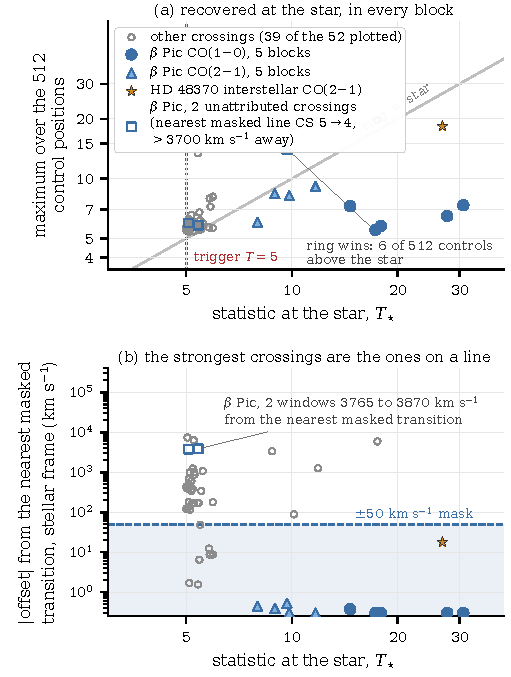
\includegraphics[width=\columnwidth]{figures/bpic_control.pdf}
\caption{The $\beta$~Pictoris positive control, in both directions. Both
panels draw the same \BpicPanelNDrawn{} of the \NCross{} crossings, the
remainder having no retained control ring. \emph{(a)}~The spatial screen:
the stellar statistic against the maximum over that window's \NCtrl{}
control positions. Filled symbols are the blocks in which the search
recovers circumstellar carbon monoxide at $\beta$~Pictoris,
\NStageOneBpicEb{} of them with the star above every control and one with
the ring above it, block \texttt{\BpCtrlBlock}, Band~\BpCtrlBand, where the
ring reaches \BpCtrlRingMax{} against \BpCtrlStar{} at the star
(\S\ref{sec:bpicval}). \emph{(b)}~The same crossings by velocity offset
from the nearest masked transition \emph{in their own star's rest frame},
with the adopted $\pm\MaskHalfKms$\,km\,s$^{-1}$ half-width marked: the
\BpicPanelNCo{} $\beta$~Pictoris carbon-monoxide crossings land
\BpicDvCoLo--\BpicDvCoHi\,km\,s$^{-1}$ from CO, while its
\BpicPanelNCs{} unattributed crossings lie
\BpicDvCsLo--\BpicDvCsHi\,km\,s$^{-1}$ from the nearest transition the
mask holds, CS($5{\to}4$). \BpicPanelNOther{} further crossings are grey,
HD~48370 marked.}
\label{fig:bpiccontrol}
\end{figure}
